\section{Поиск элементов}

\subsection{Повороты на $0 \land \ \cfrac{\pi}{3} \land \ \cfrac{2 \pi}{3}$}

Сначала найдем чевидные элемнты группы это повороты на 
$0 \land \ \cfrac{\pi}{3} \land \ \cfrac{2 \pi}{3}$ вогруг осей проходящих через 
высоту падающай из произвольной вершины. Таик такую группу 
повротов мы уже знаем это $C_3^n$ приэтом заметим что для любой вершины 
еденичные элемнты будут совпадть поэтому всего повротов будет $4*3 = 8$. 
Еслри пронумеровать вершины то можем обозначить элемнты ледующим обзазам

\begin{eqnarray}
    C_3^{n \ v}, \ n \in \insqr{1, 2}, \ v \in \insqr{0, 1, 3, 4}
\end{eqnarray}

\begin{figure}[H]
    \centering
    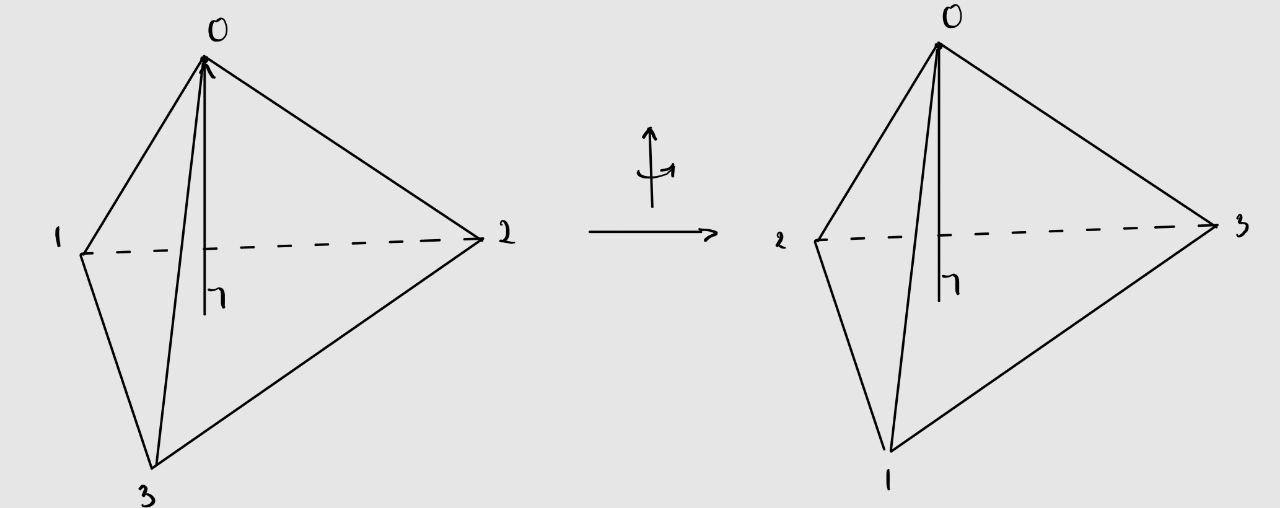
\includegraphics[width=0.5\linewidth]{su/C_10_3.jpg}
    \caption{Действие элемента $C^{1 \ 0}_{3}$}
\end{figure}

\subsection{Повороты на $\pi$}

Такжем можем легко заметить что есть повороты на $\pi$ вокруг оси соединяющей
середины противоположных ребер. Тоесть для всего таких элементов $6/2 = 3$, 
делю на 2 тк для ребрер $e_1 e_2$ и $e_2 e_1$ один и тот же.  Обозначим их так:

\begin{equation}
    C_{2}^{e_1 \ e_2} = C_{2}^{e_2 \ e_1} = C_{2}^{e_1} , \ e_1, e_2 \in \inner{01, 02, 03, 12, 13, 23}
\end{equation}

\begin{figure}[H]
    \centering
    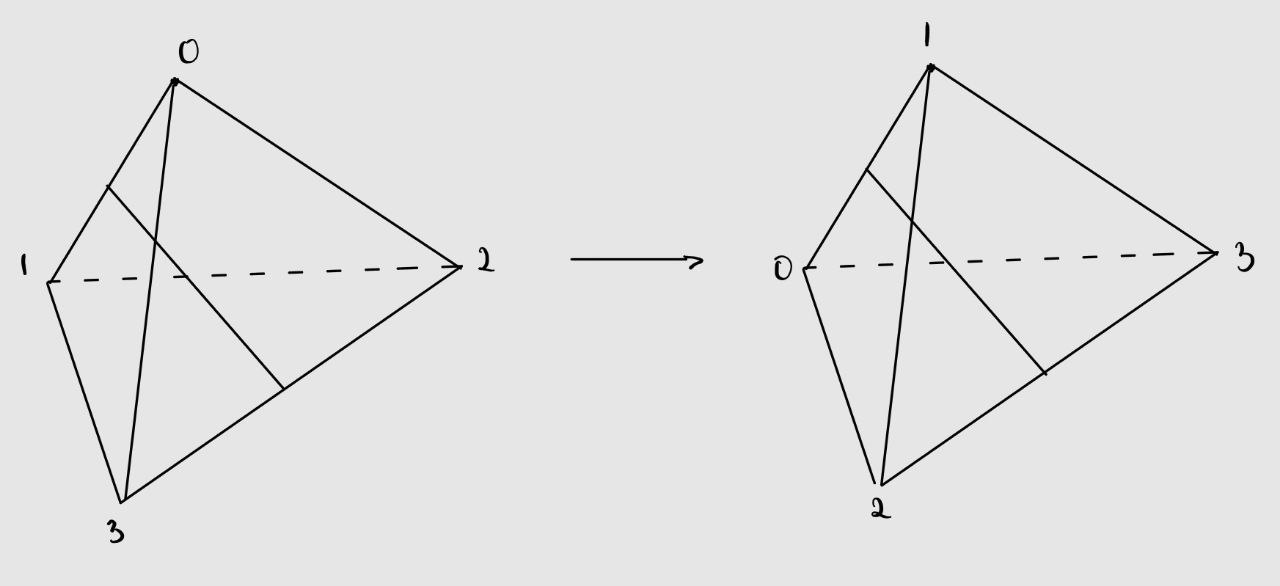
\includegraphics[width=0.5\linewidth]{su/C_15_2.jpg}
    \caption{Действие элемента $C^{01}_{2}$}
\end{figure}

\subsection{Отражения}

И самое последнее, что можно легко зметить это отраженияо тносительно плоскости 
оразуемой ребром и серединой протипротоволежащего ребра. Таким образом всего 
элементов будет $6$ - количество ребер. Введем следующее обозначения:

\begin{equation}
    \sigma^{e_1}, e_1 \in \inner{01, 02, 03, 12, 13, 23}
\end{equation}

\begin{figure}[H]
    \centering
    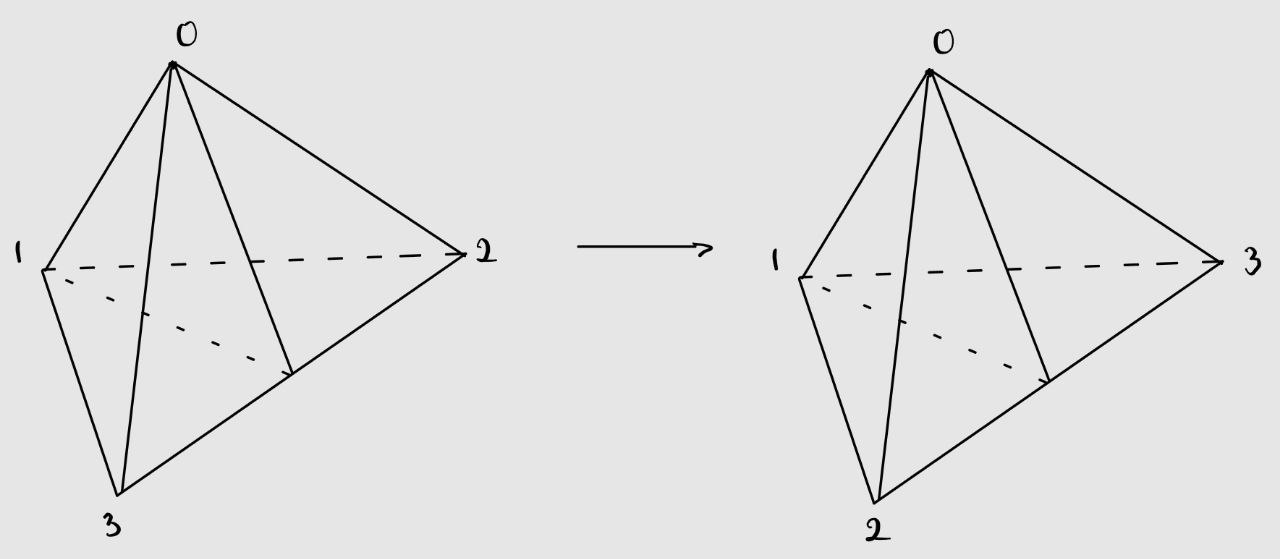
\includegraphics[width=0.5\linewidth]{su/sigma_01.jpg}
    \caption{Действие элемента $\sigma^{01}$}
\end{figure}

\subsection{Дополнение до группы}
Как можно заметить пака что элементов меньше чем требуется, поэтому пред оставлю 
машине посчитаь за меня оставшиеся элементы. Но перед этим я зметил что
группу сииметрий тетраидера и вроде как любой фигуры (для тетраидера и 3Д 
фигур точно работает), можно задать изоморфизм на подгуппу кос (без учета 
нахлеста) с количеством нитей равным количеству вершин фигуры. 
Тоесть можем перписать наши эленты следующи образом:

\begin{eqnarray}
    e &\to &0123\\
    C_3^{1 \ 0} &\to & 0231 \\
    C_2^{01} &\to & 1032\\
    \sigma^{01} &\to & 0132
\end{eqnarray}

Думаю изорфизм остальных элементов очевиден. Следствем такого изоморфизма 
является тот факт, что моя группа э то Гуппа престановок 4 элемнтов $\inner{S_4}$
Тут же заметим простой факт элементы из $C_3$ это циклическая перстановка 3 элементов, $C_2$ - перстановка 
элентов внутри 2х пар, $\sigma$ перестановка элемнтов внутри одной пары. 
Можно леко дополнить группу протой найдя оставшиеся перстаовки,
но я написал код так, что омотри код.

В итоге получу полную группу $T_d=$ (0123, 1032, 2301, 3210, 0231, 
0312, 2130, 3102, 1320, 3021, 1203, 2013, 0132, 0321, 0213, 3120, 2103, 
1023, 1230, 1302, 2031, 3012, 2310, 3201)

